\documentclass[17pt]{extarticle}
\usepackage{tikz}
 \usepackage{array}
 \usepackage{showexpl}
\lstset{
	basicstyle=\ttfamily\scriptsize,
	tabsize=2,
	explpreset={pos=r,rframe={}}
}
 
\newenvironment{MyTableEnvi}[2]
{
\newcolumntype{C}{m{#1\linewidth}}
\newcolumntype{D}{>{\scriptsize\centering\arraybackslash}m{#2\linewidth}}
\ignorespaces
\begin{tabular}{|C|D|} 
\hline	
}
{
\end{tabular}
}
 
\begin{document}
 
\begin{MyTableEnvi}{0.5}{0.5}
%%%% FIRST ROW
\begin{LTXexample}[pos=b,preset=\centering,width=0.5\linewidth]
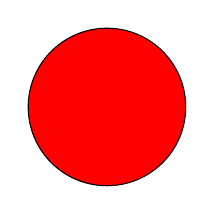
\begin{tikzpicture}
    \draw[fill=red] (0,0) circle (1);
\end{tikzpicture}
\end{LTXexample}
&
\begin{LTXexample}[pos=b,preset=\centering,width=0.5\linewidth]
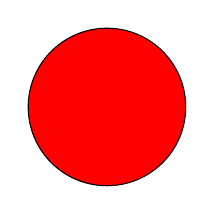
\begin{tikzpicture}
    \draw[fill=red] (0,0) circle (1);
\end{tikzpicture}
\end{LTXexample}

\\ \hline
%%%% SECOND ROW 
\begin{LTXexample}
\[
\frac{dy}{dx}=\cos x
\]
\end{LTXexample}
&
Derivative\\ \hline
\end{MyTableEnvi}


\pagebreak


 
\end{document}
